\parindent=0em
\subsection{Magic Leap One}
\noindent

El dispositivo \textit{Magic Leap One}\footnotemark~(figura~\ref{fig:vistasMagicLeapnOne}) fue lanzado al mercado en el año 2018 de manos de la compañía Magic Leap. Principalmente este casco destaca por su ligero peso de 316g frente a otros dispositivos, por otra parte, son un HMD independiente ya que viene con un sistema (procesador y tarjeta gráfica) para no tener que ser usado mediante conexión con un ordenador. Aunque no es necesario conectarlo al ordenador, el dispositivo tiene conexión \textit{bluetooth}, WiFi y USB para poder conectarse al PC y manejar archivos o instalar aplicaciones.\\

\footnotetext{Especificaciones: \href{https://www.businessinsider.com/magic-leap-one-creator-edition-price-specifications-battery-life-release-date-2018-8}{\nolinkurl{https://www.businessinsider.com/magic-leap-one}}}

Por otra parte, pese a que dispone de tecnología de \textit{hand tracking}, viene con un mando para simular una de las manos del usuario, asimismo, utiliza la tecnología de \textit{eye tracking} para poder interactuar con el entorno a través de la mirada. Del mismo modo, el dispositivo captura 6DoF, tiene un campo de visión de 50\degree  y una resolución de 1.280x960 píxeles por ojo (un total de 2.560x960 píxeles en combinación con los dos ojos).
 

\begin{figure}[htbp]
\centering
    \hspace{-4mm}
    \begin{minipage}{0.5\textwidth}
        \centering
        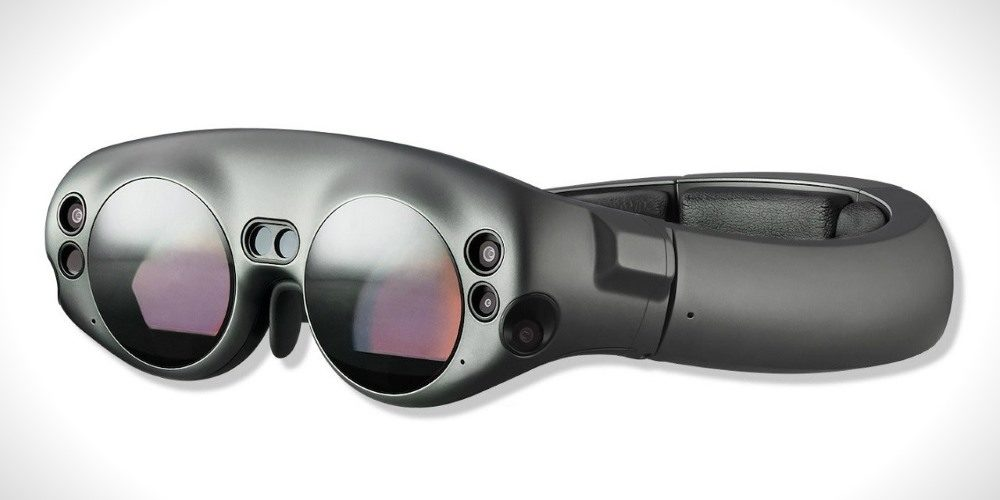
\includegraphics[scale=0.8]{Images/Estado del arte/magicleapone1.jpg}\\
        (a) Vista del casco completo
    \end{minipage}
    \begin{minipage}{0.5\textwidth}
        \centering
        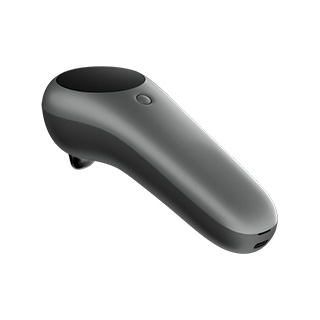
\includegraphics[scale=0.3]{Images/Estado del arte/magicleapone2.jpg}\\
       (b) Vista del mando
    \end{minipage}\\
    \caption[Dispositivo completo de las \textit{Magic Leap One}]{Dispositivo completo de las \textit{Magic Leap One}\footnotemark.}
    \label{fig:vistasMagicLeapnOne}
\end{figure}
\footnotetext{Fuente: \href{https://www.estiloextra.net/magic-leap-one-las-nuevas-y-prometedoras-gafas-de-realidad-aumentada/}{\nolinkurl{https://www.estiloextra.net/magic-leap-one}}}


Por último, la batería recargable de litio de las \textit{Magic Leap One} permite un uso continuado de 3 horas y, además, tiene un diseño ergonómico mediante el cual se puede utilizar el casco con gafas, ya que hay un compartimento enfrente de los ojos adaptado para dicho uso.

%https://www.businessinsider.com/magic-leap-one-creator-edition-price-specifications-battery-life-release-date-2018-8?IR=T

